\documentclass[fleqn]{ctexart}
\usepackage{graphicx}
% 数学支持（提供 \mathbb、\dfrac 等）
\usepackage{amsmath,amssymb}
% 页面与版式设置：更小的页边距与顶部空白
\usepackage[a4paper,top=15mm,bottom=20mm,left=12mm,right=12mm]{geometry}
% 自动换行与字偶距优化
\usepackage{microtype}
\microtypesetup{tracking=true,protrusion=true,final}
% 在需要时放宽断行以避免溢出（数值可按需调整）
\setlength{\emergencystretch}{2em}
% 列表控制，便于让(1)后直接跟内容
\usepackage{enumitem}
% 使章节标题左对齐（同时保留 ctex 默认样式）
\ctexset{section={format+=\raggedright}}
%1.3倍行距
\renewcommand{\baselinestretch}{1.3}
% 数学左对齐缩进为0
\setlength{\mathindent}{0pt}
% 增大矩阵的行距
\renewcommand{\arraystretch}{1.3}
\pagestyle{empty}
\begin{document}
\section*{题目1}
% 写一段代码
\begin{verbatim}
void foo(int n) {
	int i;
	for (i = 0;i<n;i++)
		Fork();
	printf("hello\n");
	exit(0);
}
\end{verbatim}

\medskip
应用枚举法，$n=0$时1个进程，输出1个“hello”，$n=1$时有2个进程，输出2个“hello”，$n=2$时有4个进程，输出4个“hello”，而$n=3$时有8个进程，输出8个“hello”，因此当$n$时有$2^n$个进程，输出$2^n$个“hello”。

\section*{题目2}
\begin{verbatim}
Int main() {
	if (fork() == 0) {
		printf(“a”);	fflush(stdout);
		exit(0);
	}else {
		printf(“b”);	fflush(stdout);
		waitpid(-1, NULL, 0);
	}
	printf(“c”);	fflush(stdout);
	exit(0);
}
\end{verbatim}

\medskip
子进程会输出“a”，父进程会输出“b”和“c”，但需要注意的是父进程的waitpid函数会使它等子进程结束后再继续执行，因此可能的输出为“abc”或“bac”

\section*{题目3}
\begin{verbatim}
#include “csapp.h” 
int main() { 
	int x = 3;
    if (Fork() != 0) 
		printf("x=%d\n", ++x); 
	printf("x=%d\n", --x); exit(0); 
} 
\end{verbatim}

\medskip
父进程会输出“4”和“3”，子进程会输出“2”，因此可能的输出为“243”“423”“432”（我省略了“$x=$”）

\section*{题目4}
\begin{verbatim}
    #include “csapp.h”
void end (void) {
	printf(“2”); fflush(stdtou);
}
Int main() {
	if(Fork() == 0) 
		atexit(end);
	if(Fork() == 0) {
		printf(“0”);
        fflush(stdout);
	}else {
		printf(“1”);
		fflush(stdout);
	}
	exit(0);
}
\end{verbatim}

\medskip
%插入一张图片，紧挨着上面的部分并居中
\begin{center}
    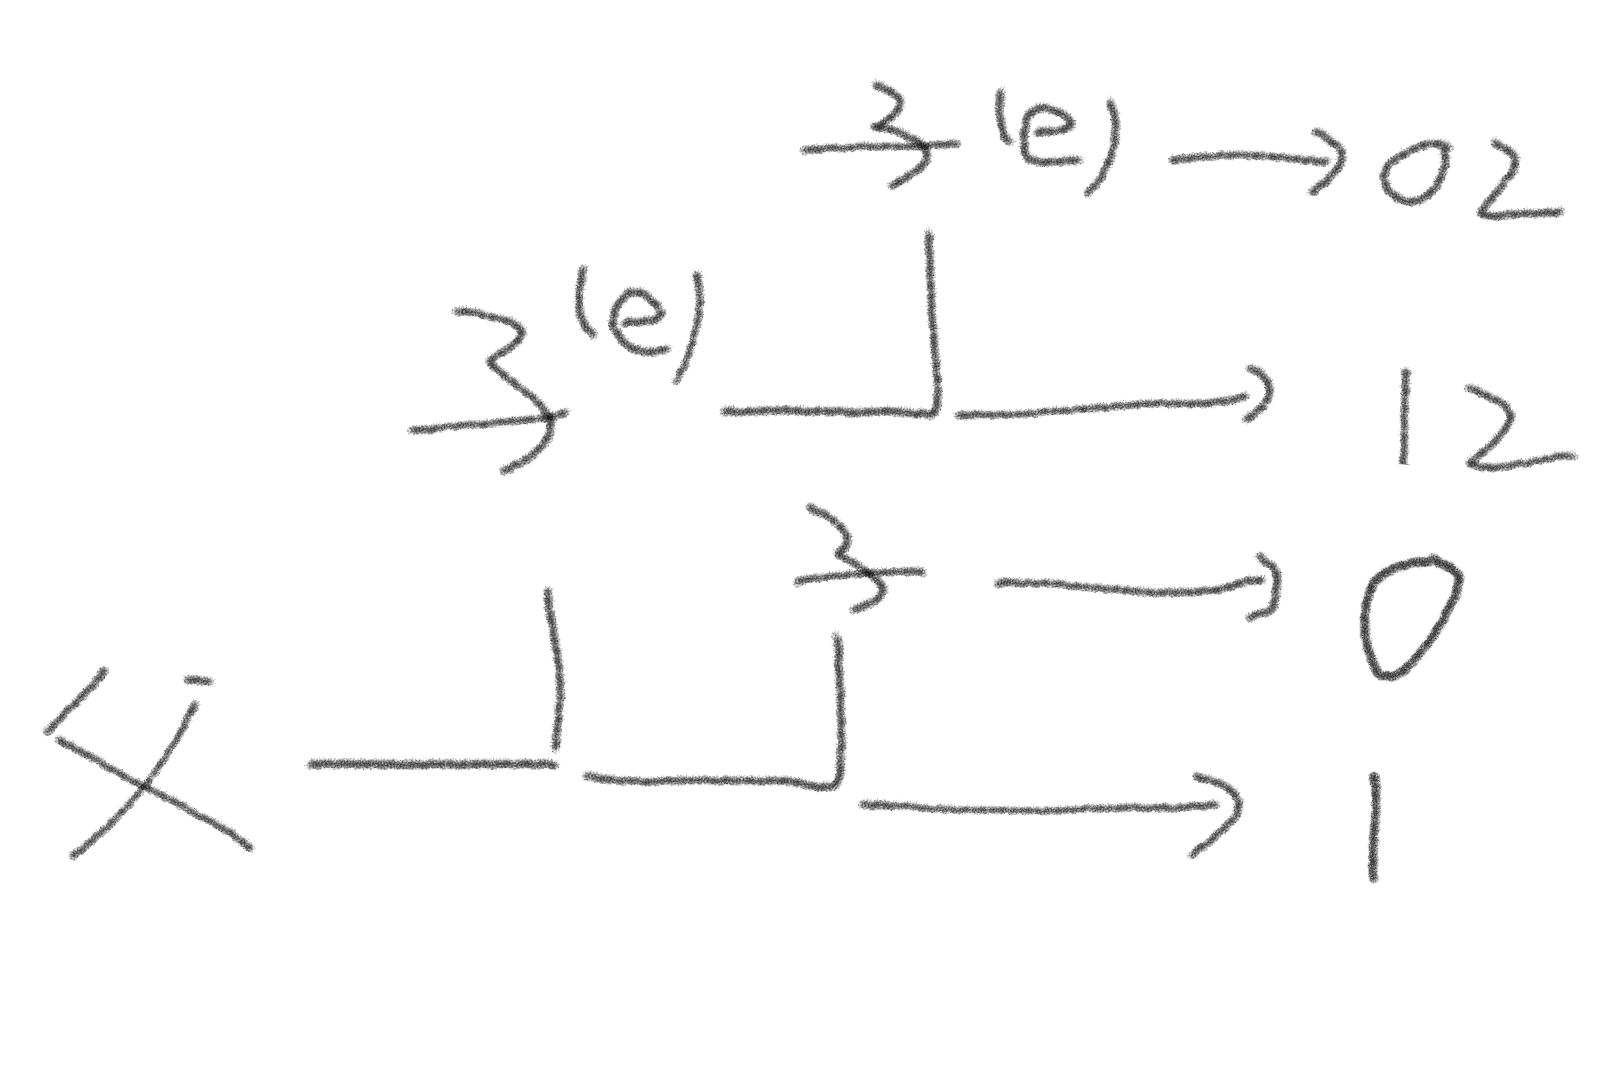
\includegraphics[width=0.5\textwidth]{示意图.jpg}
\end{center}

\medskip
根据我的草稿，输出为“02”“12”“0”“1”自由排列，因此可以选出A、C、E作为可能的输出
\end{document}